%\typeout{IJCAI-15 Instructions for Authors}

\documentclass{article}
% The file ijcai15.sty is the style file for IJCAI-15 (same as ijcai07.sty).
\usepackage{ijcai15, graphicx, times, flushend}
\usepackage[ruled,vlined]{algorithm2e}

\SetAlgoCaptionSeparator{.\space}
\renewcommand\AlCapFnt{\normalfont\scshape}
\setlength{\algomargin}{0.7cm}

\title{GraphEvol: A Graph Evolution Technique for Web Service Composition}

\author{Alexandre Sawczuk da Silva, Hui Ma, Mengjie Zhang\\ School of
Engineering and Computer Science, Victoria University of Wellington, New Zealand\\
\{Alexandre.Sawczuk.da.Silva, Hui.Ma, Mengjie.Zhang\}@ecs.vuw.ac.nz}

%\author{Qiang Yang \\
%Hong Kong University of Science and Technology\\
%Hong Kong, China \\
%pcchair15@ijcai.org}

\begin{document}

\maketitle

\begin{abstract}
  Web service composition can be thought of as the combination of reusable functionality modules available over the network to
  create applications that accomplish more complex tasks. Evolutionary Computation (EC) techniques have been applied with success
  to the problem of fully automated Web service composition, which is when candidate services are selected at the same time that the best configuration in which to connect those candidates is determined. However, all of
  these techniques encode candidate solutions, which can be naturally thought of as Directed Acyclic Graphs (DAGs), into some  
  other representation, commonly trees. This paper proposes GraphEvol, an evolutionary technique that investigates the direct use
  of DAGs to represent and evolve Web service composition solutions. GraphEvol is analogous to Genetic Programming (GP), but 
  implements the mutation and crossover operators differently. Experiments were carried out comparing GraphEvol to a GP technique
  for a series of composition tasks, with results showing that GraphEvol solutions either match or surpass the quality of those 
  obtained using GP, requiring equal or less execution time.
\end{abstract}

\section{Introduction}

\begin{figure}
\centerline{
\fbox{
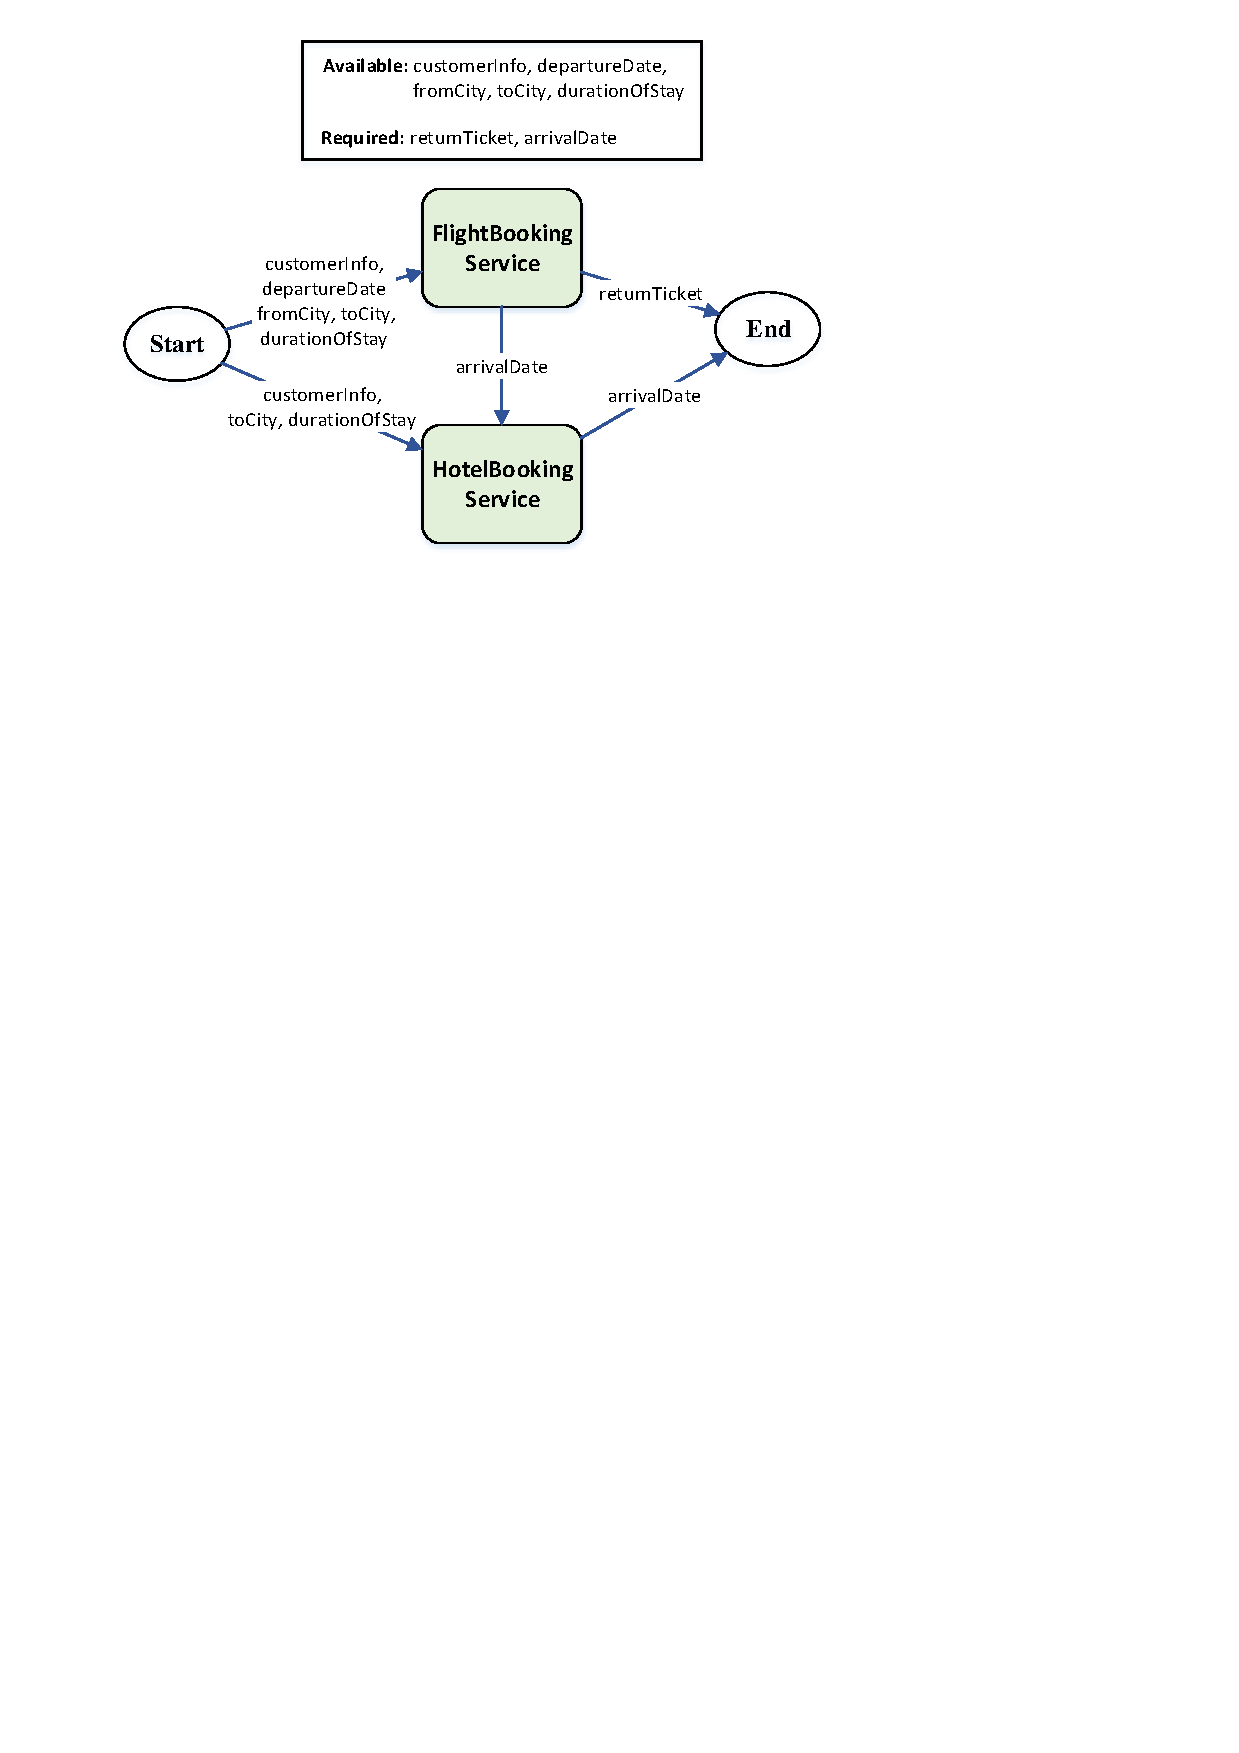
\includegraphics[width=8cm]{compositionExample.pdf}}}
\caption{Example of a solution to a Web service composition task.}
\label{fig:compositionExample}
\end{figure}

A Web service can be defined as a software module that accomplishes a specific task and that is made available for requests over
the Internet \cite{gottschalk2002introduction}. The fundamental benefit of such modules is that they can be interwoven with new applications, preventing developers from rewriting
functionality that has already been implemented. Service-Oriented Architecture (SOA) is a paradigm that expands on this idea, advocating
that the main atomic components of a software system should be Web services, since this maximizes code reuse and information sharing \cite{perrey2003service}.
As services are typically present standard interfaces, the possibility arises to create approaches capable of combining services
automatically according to the final desired system, in a process known as \textit{Web service composition} \cite{milanovic2004current}. The objective of these approaches
is to produce a workflow, i.e. a directed acyclic graph (DAG), stipulating the sequence in which each atomic service should be executed, as well as
the output-input connections between services.

Many approaches to Web service composition have been proposed in the literature, from variations on AI planning techniques \cite{deng2013efficient} to the employment
of integer linear programming solvers \cite{yoo2008web}. In particular, promising results have been achieved with the use of Evolutionary Computation (EC) techniques \cite{wang2012survey},
because their search methods successfully handle the large search space characteristic of the composition problem. Existing evolutionary
techniques for fully automated Web service composition can be divided into two different groups according to the extent of the composition they
perform: \textit{semi-automated composition techniques}, assume that a general workflow of abstract tasks has already been provided and that the
algorithm must simply find the best candidate for each task slot; \textit{fully automated composition techniques}, on the other hand, make no such
assumption, meaning that they construct the task workflow and select the most suitable candidates simultaneously. Because of their greater capabilities,
fully automated composition techniques are the focus of this paper.

While semi-automated composition can be accomplished using a variety of techniques such as Genetic Algorithms (GA) and Particle Swarm Optimisation
(PSO) \cite{silva2014graph}, fully automated composition using EC is currently mostly restricted to techniques employing the traditional Genetic Programming (GP) model \cite{rodriguez2010composition}.
In this paradigm, each each composition candidate is a tree that represents an underlying graph solution that can be obtained through a translation
process. The question then arises whether it is possible to represent a candidate directly as a graph, and whether the system's performance is affected
from doing so. Thus, the objective of this paper is to present and analyse \textit{GraphEvol}, an evolutionary computation technique for Web service
composition where each candidate is represented as a DAG and modified while remaining in that form. Apart from possible performance gains, the main
advantage of GraphEvol is that it represents each solution in an intuitive and direct way, allowing a more powerful way of ensuring that solutions
meet correctness constraints. The remainder of this paper is organised as follows:
Section \ref{background} presents background information concerning Web service composition; Section \ref{graphevol} presents the proposed technique;
Section \ref{experimentdesign} discusses the experiments conducted to compare the performance GraphEvol to that of a GP composition approach;
Section \ref{results} describes the experiment results; Section \ref{conclusions} concludes the paper.

\section{Background}\label{background}

\subsection{The Web Service Composition Problem}

In a standard composition problem, a user would like to obtain a composite Web service with a particular functionality. The user makes a request to a Web
service composition system specifying the \textit{inputs} the composite service should accept, the \textit{outputs} it should produce, the \textit{constraints}
it should consider (e.g. the resulting composite service should have the lowest possible execution time), and the \textit{repository} from which it should select
the atomic services to include in the composition. Given this information, the composition system \textit{discovers} relevant services from the repository, and uses
these services as potential candidates to be included in the final composition. A composition algorithm is run to \textit{select} appropriate services at the same
time it \textit{builds} a workflow denoting how each service in the composition interacts with the others with regards to their required input and produced output.

A classic example of automated Web service composition is the travel planning scenario \cite{srivastava2003web}, where the objective is to create a system capable of
automatically reserving hotels and flights according to customer preferences. In this scenario the customer preference types, such as departure date and destination
city, are the composition \textit{inputs}, and the reservation outcomes, such as issued tickets and receipts, are the composition \textit{outputs}. The relevant composition
candidates are a set of hotel and flight booking services that are to be combined into a cohesive task workflow by the composition system. Figure \ref{fig:compositionExample} shows a simple composition solution that performs flight and hotel reservations according to a customer's information. More specifically, when using this composite service 
the customer provides her/his personal information and travel details, such as the departure date, the destination city and the duration of the stay. This information is
then used to book return flight tickets, and to determine the customer's arrival date at the destination city.

\subsection{Related Work}

\begin{figure}
\centerline{
\fbox{
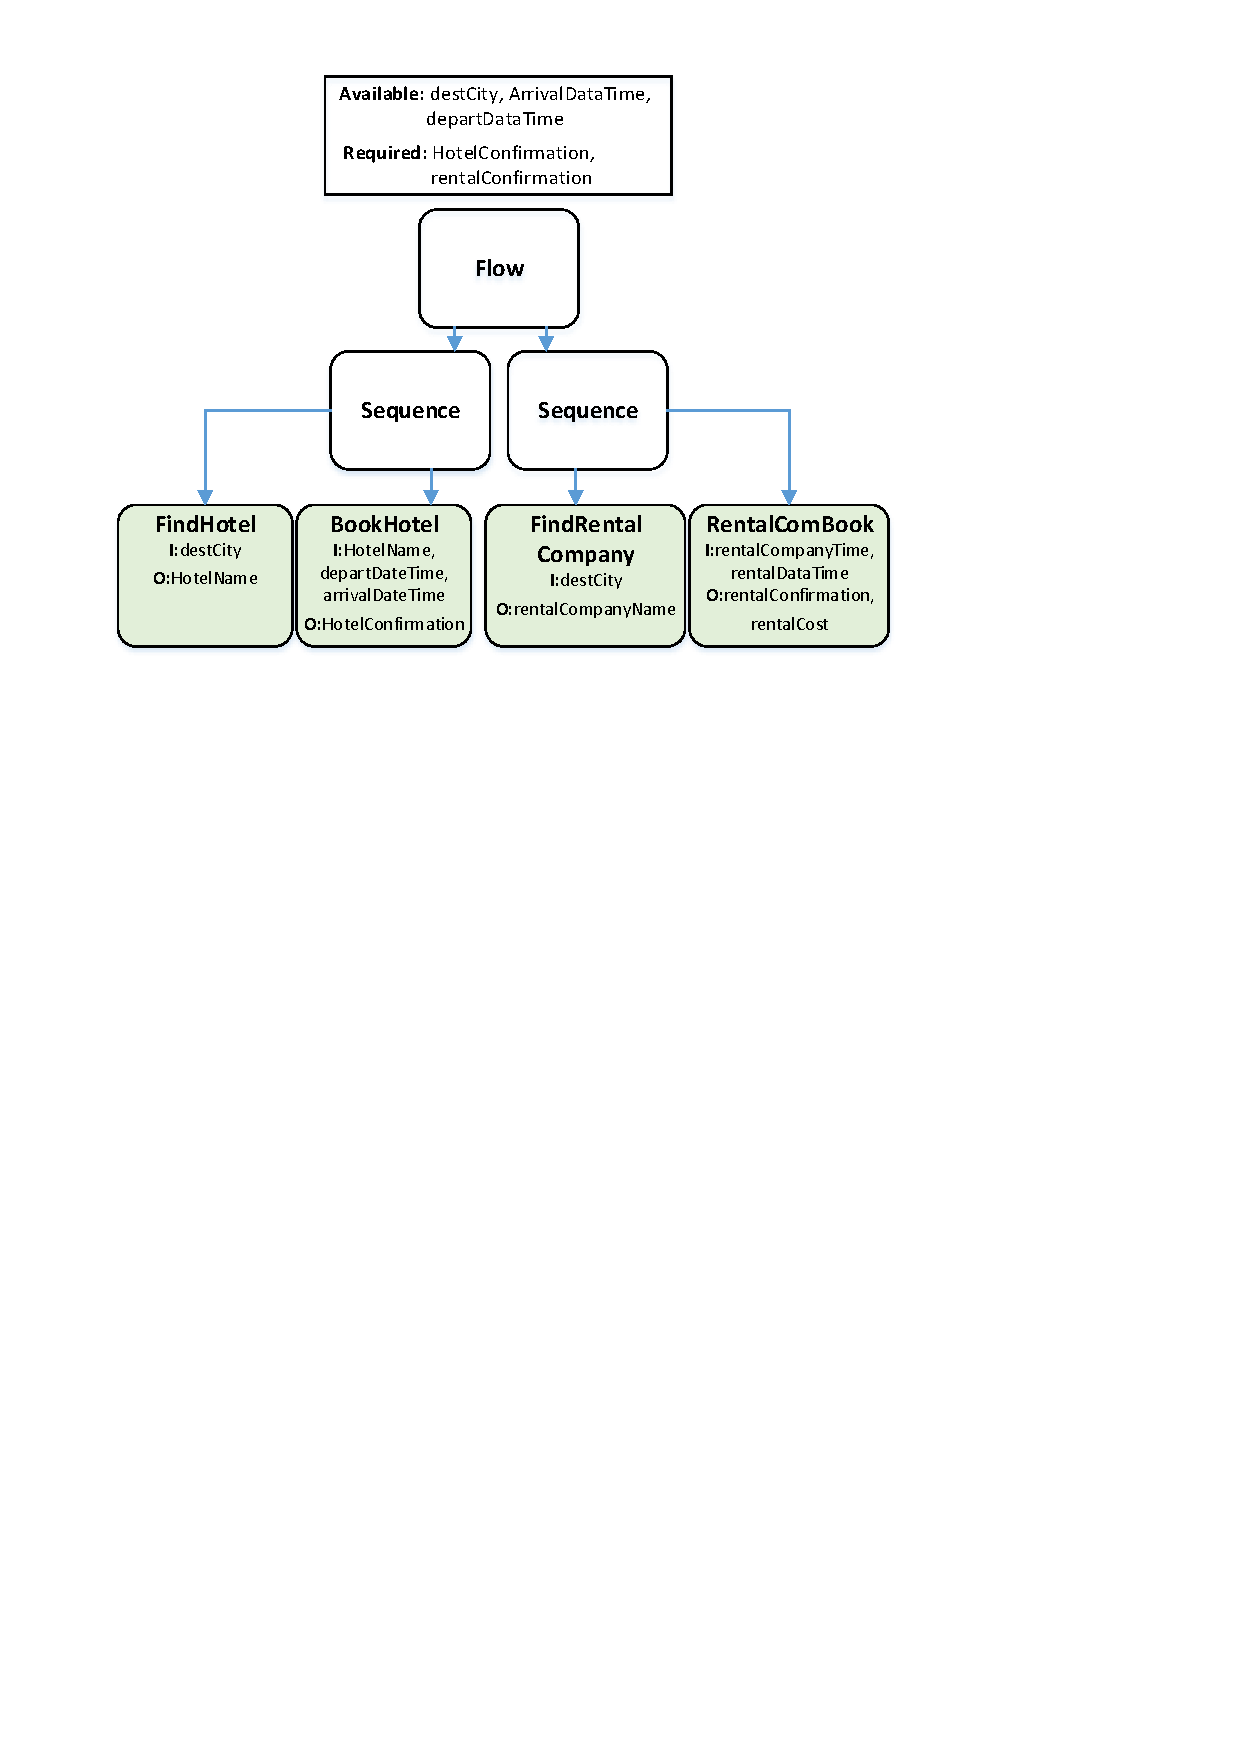
\includegraphics[width=8cm]{treeExample.pdf}}}
\caption{Example of a typical GP candidate composition tree \protect\cite{aversano2006genetic}.}
\label{fig:treeExample}
\end{figure}

There are many publications on the subject of EC applied to Web service composition, but this Subsection will focus on those which perform fully automated composition,
since their composition outcomes are analogous to those of GraphEvol. One of the pioneering GP composition approaches \cite{aversano2006genetic} uses workflow constructs as the non-terminal tree nodes and Web service candidates as the terminal nodes, where workflow constructs represent the output-input connections between
two services. For example, if two services are sequentially connected, so that output of service \textit{A} is used as the input of service \textit{B}, this would be represented
by a \textit{sequence} workflow construct having \textit{A} as the left child and \textit{B} as the right one. Likewise, if two services \textit{A} and \textit{B} have independent inputs and outputs and can be executed in parallel, this can be encoded as a \textit{flow} construct having \textit{A} and \textit{B} as its children. An example of a tree generated by this technique is shown in Figure \ref{fig:treeExample}, adapted from an illustration in the referenced work. The initial population is initialised randomly, which means that the initial compositions represented in that generation are very unlikely to be executable, since their inputs and outputs are mismatched. The aim of the technique is to improve these output-input matches by employing a fitness function that calculates their correspondence and awards higher fitness scores to those candidates with larger overlaps. The genetic operators employed for this evolutionary process are crossover, where two subtrees from two individuals are randomly selected and swapped, and mutation, where a subtree for an individual is replaced with a randomly generated substitute.

Another GP approach \cite{rodriguez2010composition} follows a similar tree representation to the one discussed above, as well as a similar implementation of mutation and crossover operators. The greatest distinction between this approach and others is in its use of a context-free grammar to generate the initial population of candidates and to create the subtrees used during mutation. The grammar restricts the tree structure configurations allowed in the tree, thus reducing the search space considered when searching for a solution. Another key difference of this approach is in its fitness function, which not only minimises the output-input mismatches in candidates, but also minimises the overall number of atomic services in the composition and the size of the largest sequential chain of such services. These two additions to the fitness function are aimed at reducing the overall execution time and cost of the resulting compositions. This technique was tested against two well-known semantically-annotated datasets, OWL-S TC \cite{kuster2008opossum} and WSC 2008 \cite{bansal2008wsc}, showing that it yields valid solutions to all composition tasks while requiring a relatively low amount of execution time.

\begin{figure}
\centerline{
\fbox{
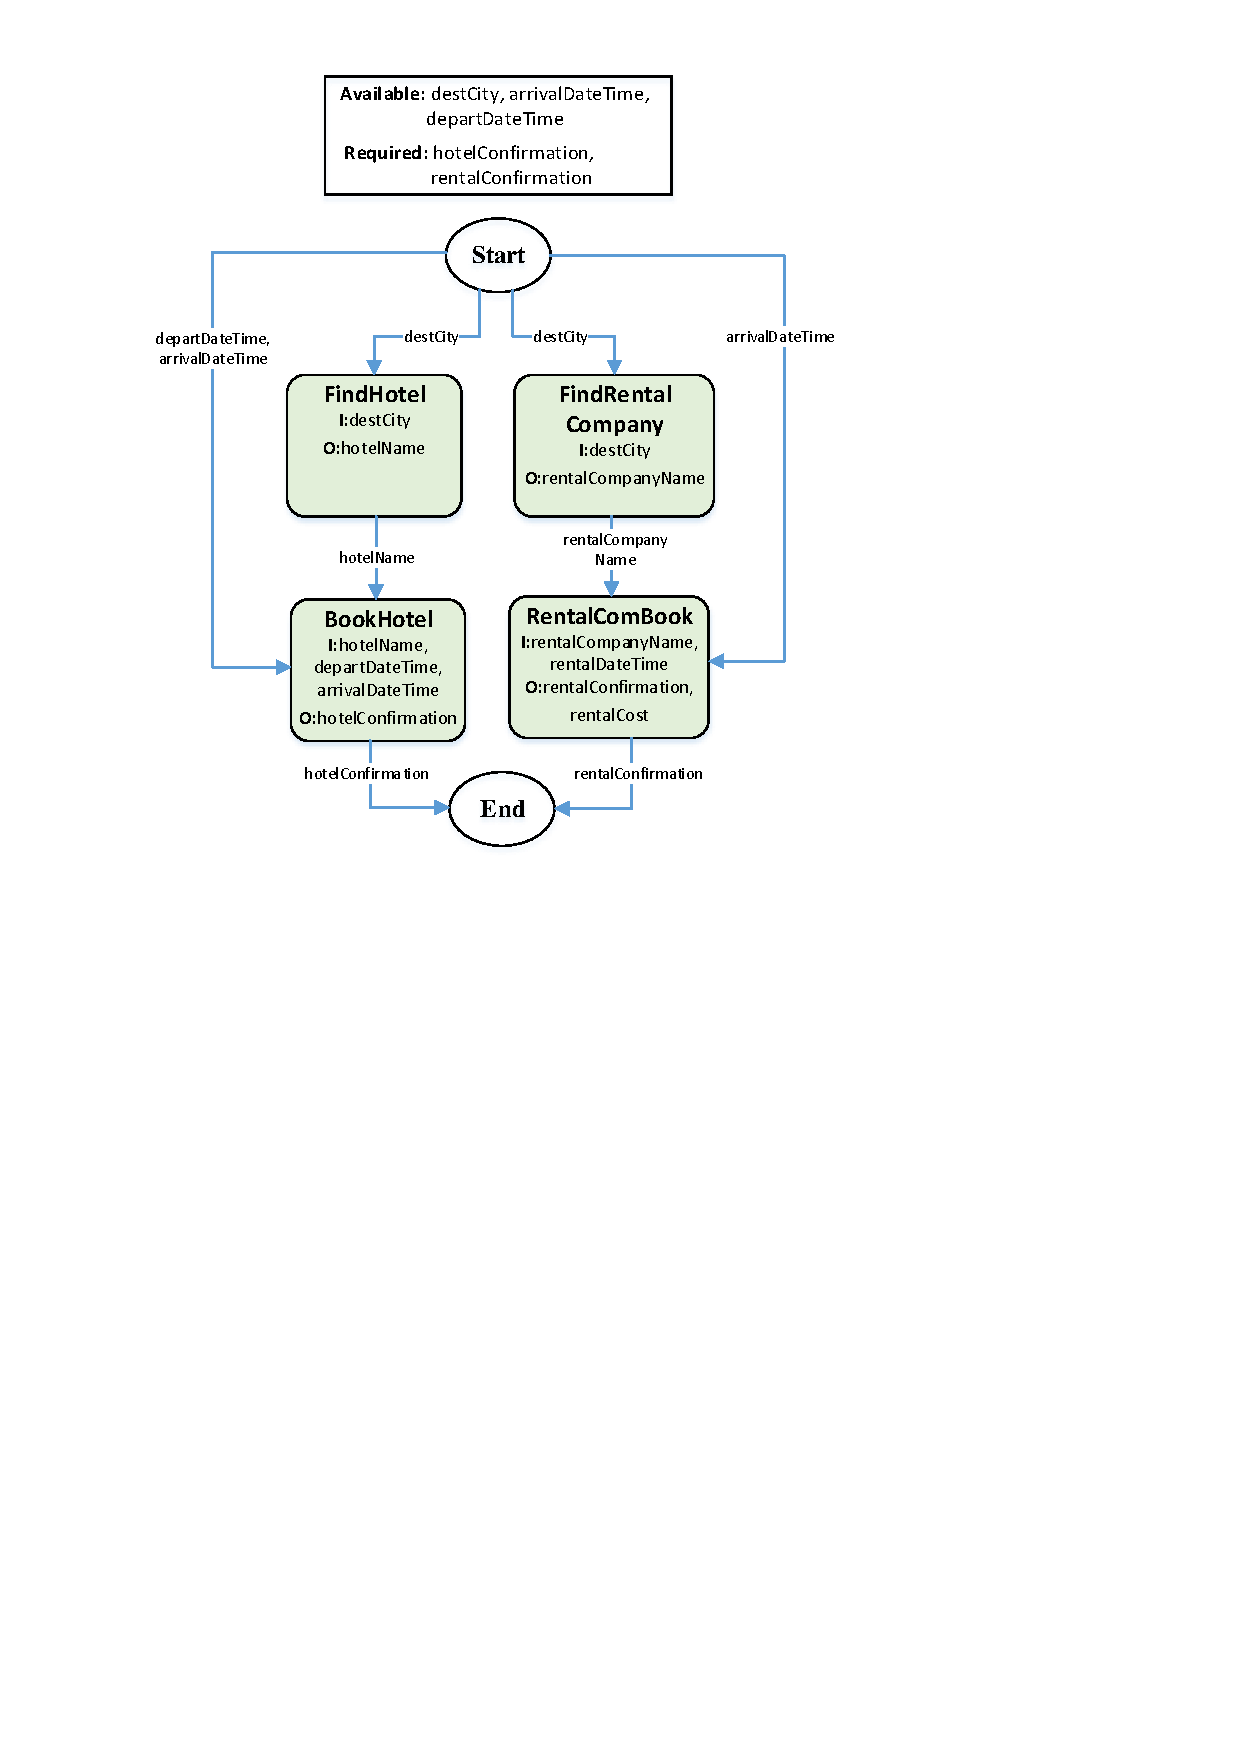
\includegraphics[width=8cm]{graphExample.pdf}}}
\caption{Example of a candidate composition in GraphEvol.}
\label{fig:graphExample}
\end{figure}

\begin{algorithm}
 \setlength\hsize{0.9\linewidth}
 \SetKwInOut{Input}{Input}\SetKwInOut{Output}{Output}
 \let\oldnl\nl% Store \nl in \oldnl
\newcommand{\nonl}{\renewcommand{\nl}{\let\nl\oldnl}}
 \LinesNumbered
	\textbf{1.} Initialise the population using the graph building algorithm.\\
	\nonl \While {max. generations not met}{
	
	\textbf{2.} Select the fittest graph candidates for reproduction.\\
	\textbf{3.} Perform mutation and crossover on the selected candidates, generating offspring.\\
	\textbf{4.} Evaluate the fitness of the new graph individuals.\\
	\textbf{5.} Replace the lowest-fitness individuals in the population with the new graph individuals.\\
	}
 \caption{\footnotesize Steps of the GraphEvol technique.}
\label{graphEvolSteps}
\end{algorithm}

In addition to GP, an approach using PSO has also been shown to be a suitable method for fully automated Web service composition \cite{silva2014graph}. In this technique, candidates encoded as a vectors of weights (particles), each ranging from 0 to 1. These weights are mapped to the edges of a \textit{master graph}, which is a data structure created at 
initialisation time to represent all the possible output-input relationships between relevant candidate services. The central idea of this technique is to utilise a greedy algorithm
to extract non-redundant functional solutions from the master graph, using the weights as guides that prioritise the choice of certain edges and nodes of the structure. The weights
are evolved using the classical PSO algorithm, and at each generation the fitness of all solutions is calculated by extracting the underlying structure from the master graph. Since
the master graph structure is built ensuring full matching of services inputs and outputs, the fitness function employed for evolution optimises the population according to non-functional quality (QoS) measures such as response time, availability, and reliability.

\section{GraphEvol}\label{graphevol}
GraphEvol, the evolutionary computation approach proposed in this work, bears many similarities with the GP approaches discussed above. Namely, it initialises and a population 
of candidates that are encoded using non-linear data structures, evolves this population using crossover and mutation operators, and evaluates the quality of each candidate
based on the nodes included in its structure. However, as opposed to representing candidate compositions as trees that correspond to underlying graph structures, GraphEvol
represents them directly as graphs with Web service nodes. Figure \ref{fig:graphExample} shows a graph representation example that is equivalent to the candidate tree shown in Figure \ref{fig:treeExample}. As a consequence of this direct graph representation, the mutation and crossover operators must be implemented differently, and so must the fitness function. Another important aspect of GraphEvol is that is uses a graph-building algorithm for creating new  solutions, and for performing mutation and crossover. The general procedure for GraphEvol is shown in Algorithm \ref{graphEvolSteps}, however each fundamental aspect of the proposed technique is explored in more detail in the following subsections.

\subsection{Graph building algorithm}

\begin{figure}
\centerline{
\fbox{
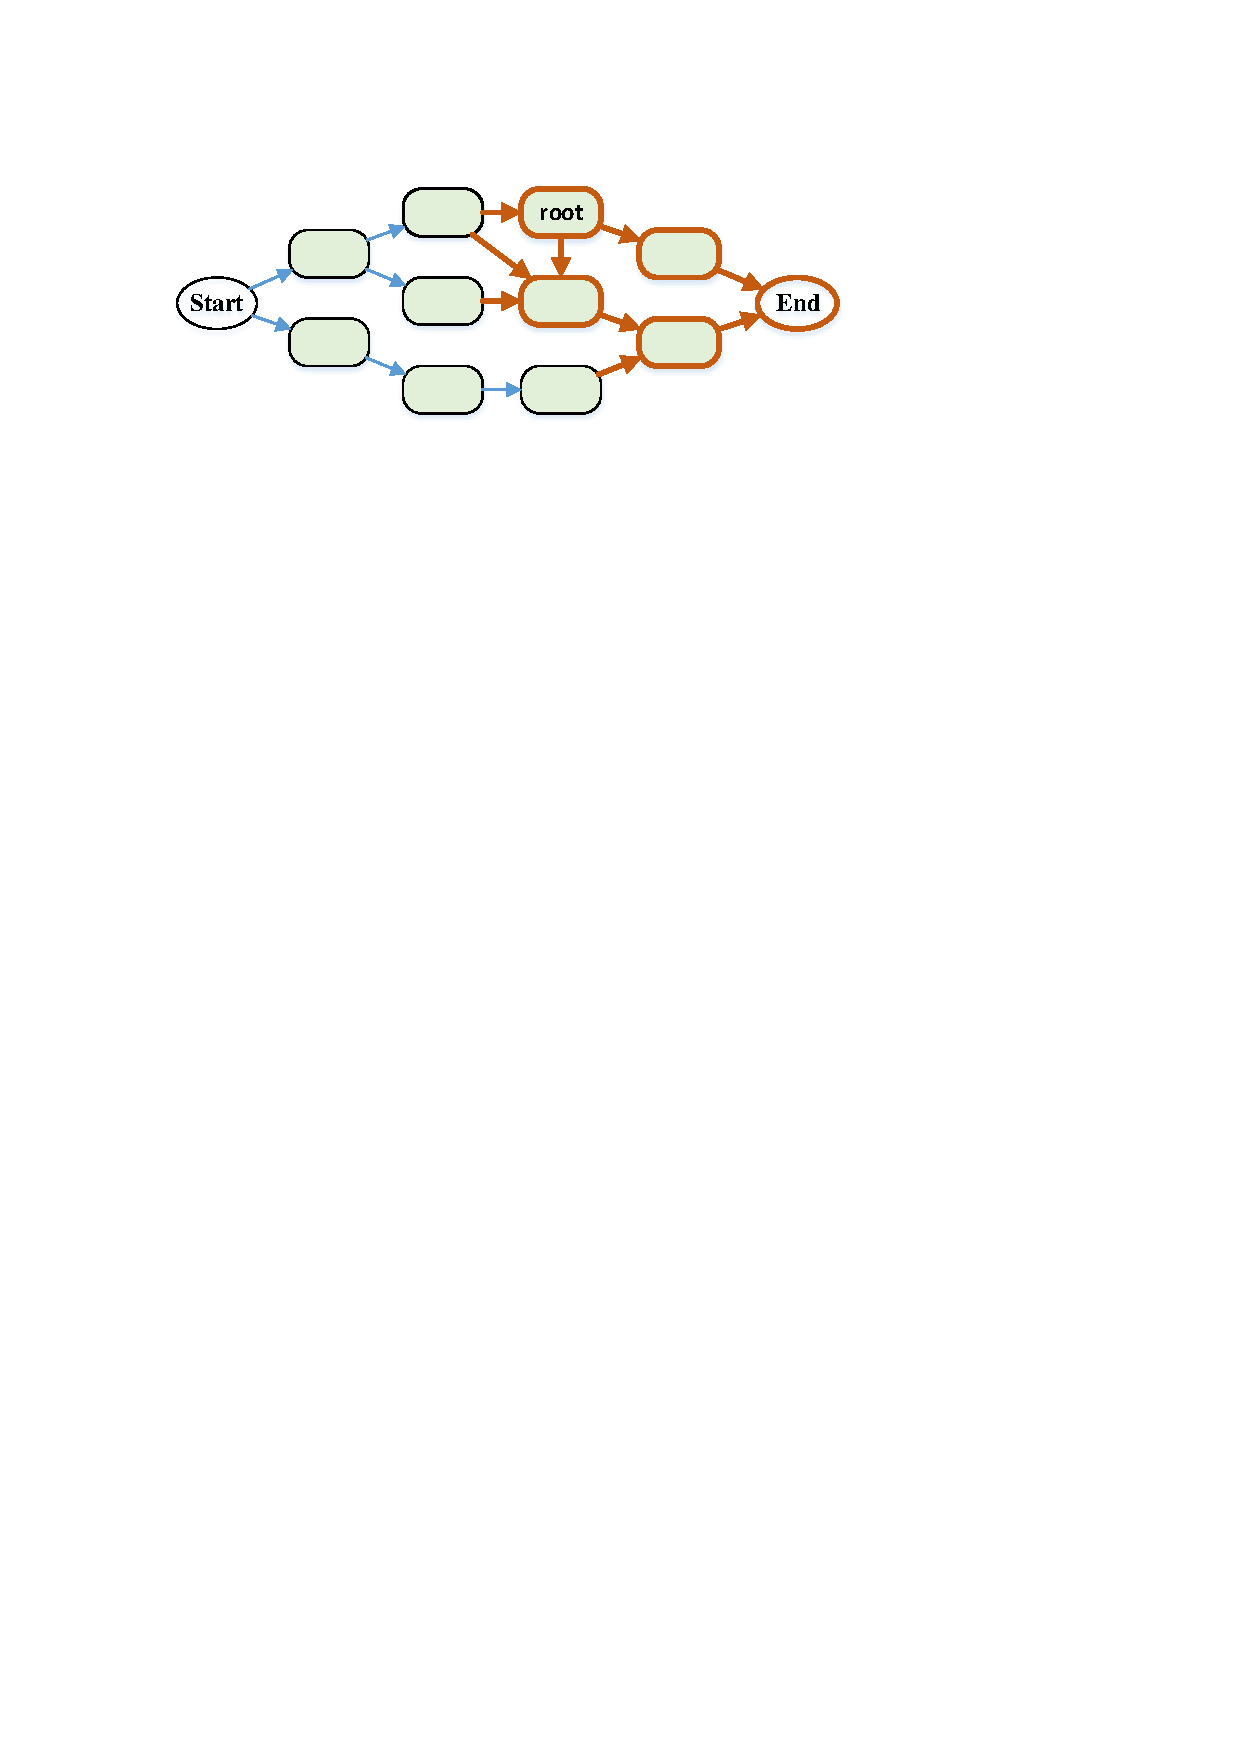
\includegraphics[width=8cm]{mutationExample.pdf}}}
\caption{Example of nodes and edges marked for deletion during the graph mutation operation.}
\label{fig:mutationExample}
\end{figure}

The initialisation of candidates is performed by employing a graph-building algorithm that is based on
the planning graph approach discussed in the composition literature \cite{chen2014qos,deng2013efficient,huang2009effective}.
At first, an algorithm is run to filter all services that will be potentially useful when building a solution, similar
to the one presented in \cite{wang2013genetic}. These relevant services, along with the composition's desired inputs and outputs, are
then presented to Algorithm \ref{generation}, whose task is to connect some of these nodes and form a non-redundant functionally
correct solution (i.e. a solution where all service inputs and composition outputs are fulfilled without any superfluous connections
between services).

\begin{algorithm}
 \setlength\hsize{0.9\linewidth}
 \SetKwInOut{Input}{Input}\SetKwInOut{Output}{Output}
 \SetKwFunction{connectNode}{connectNode}\SetKwFunction{findCands}{findCands}\SetKwFunction{removeDangling}{removeDangling}
 \LinesNumbered
 \SetNlSty{}{}{:}
 \Input{$I$, $O$, $relevant$}
 \Output{candidate graph $G$}
 $start.outputs \leftarrow \{I\}$\;
 $end.inputs \leftarrow \{O\}$\;
 $G.edges \leftarrow \{\}$\;
 $G.nodes \leftarrow \{start\}$\;
 $seenNodes \leftarrow \{start\}$\;
 $currEndInputs \leftarrow \{start.outputs\}$\;
 $candidateList \leftarrow$ \findCands{$seenNodes, relevant$}\;
 \While{$end.inputs \not\sqsubseteq currentEndInputs$}{\label{buildingLine}
 $cand \leftarrow candidateList.next()$\;
 \If{$cand \not\in seenNodes \wedge cand.inputs \sqsubseteq currEndInputs$}{
 \connectNode{$cand, G$}\;
 $currEndInputs \leftarrow currEndInputs \cup \{cand.outputs\}$\;
 $seenNodes \leftarrow seenNodes \cup \{cand\}$\;
 $candidateList \leftarrow candidateList \cup$ \findCands{$seenNodes, relevant$}\; 
 }}
 \connectNode{$end, G$}\;
 \removeDangling{$G$}\;
 \KwRet $G$\;
 \vspace{2mm}
 \SetKwProg{myproc}{Procedure}{}{}
 \myproc{\connectNode{$n, G$}}{
  $G.nodes \leftarrow G.nodes \cup \{n\}$\;
   $inputsToFulfil \leftarrow \{cand.inputs\}$\;
 \While{$|inputsToFulfil| > 0$}{
	$graphN \leftarrow G.nodes.next()$\; 
	\If{$|n.inputs \sqcap graphN.outputs| > 0$}{
	  $inputsToFulfil \leftarrow inputsToFulfil - (n.inputs \sqcap graphN.outputs)$\;
	  $G.edges \leftarrow G.edges \cup \{graphN \rightarrow n\}$\;
    }
 }}
 \caption{\footnotesize Generating a new candidate graph.}
\label{generation}
\end{algorithm}

Algorithm \ref{generation} builds the graph from the \textit{start} to the \textit{end} node, thus preventing the formation of cyclical
structures. It begins by adding the \textit{start} node to the graph, marking it as one of the
\textit{seenNodes}, and adding some initial candidates to the \textit{candidateList} to be considered for connection. These candidates
are identified using the \textit{findCands} function, which discovers which elements from the \textit{relevant} set have at least some
of their input satisfied by the nodes already in the graph (i.e. the \textit{seenNodes}). Then, the building process begins, continuing
as long as the composition outputs represented in \textit{end.inputs} have not been fulfilled by the currently available graph outputs
in \textit{currentEndInputs}. In this process, a candidate \textit{cand} is selected at random from the \textit{candidateList}, and if
it has not already been used in the graph and all of its inputs can be fulfilled by the currently available graph outputs, then it is
connected to the graph using the \textit{connectNode} function. This function identifies a random, minimal set of edges connecting the
new node (\textit{n}) to already existing nodes in the graph so that the inputs of this new node are fully satisfied. After connecting
\textit{cand} to the graph, it is added to the set of \textit{seenNodes} and the \textit{candidateList} is updated to include services
that may be fulfilled by the outputs of \textit{cand}. Finally, once the composition's required output has been reached, the \textit{end}
node is connected. This particular graph building algorithm often results in \textit{dangling nodes}, which are chains of nodes that are
connected to the graph but whose output is not used to fulfil any other nodes. Because of this, a routine to remove such chains (\textit{removeDangling})
is executed on the graph before producing the completed structure. It is important to highlight that the selection of each candidate
to connected with the graph, as well as the edges that should be used in this connection, is done stochastically, meaning that the
resulting graph varies with each run of the algorithm.

\subsection{Mutation}

Intuitively, the mutation operator for a graph candidate implements the same idea of the corresponding tree
operator \cite{aversano2006genetic}: a subpart of the candidate should be removed and replaced with a new randomly generated fragment, all
the while maintaining the functional properties of the original subpart (i.e. correct output-input matches where
the subpart connects with the main part of the candidate). To do so, we begin by randomly selecting a node in the
graph (excluding the end node) to act as the `root' of the subpart to be replaced. Subsequently, all nodes that
are directly or indirectly dependent on the outputs of this root are also identified, all the way to the end node,
as shown in Figure \ref{fig:mutationExample}. These nodes are removed from the graph, and all of its connections (edges) to the main
part of the graph are severed. Finally, the incomplete graph is fed into Algorithm \ref{generation}, but beginning
execution from line \ref{buildingLine}. This completes the graph and results in an offspring with the same main
part as its parent, but with a distinct subpart.

\subsection{Crossover}

Traditionally, the crossover operation involves the exchange of genetic material by two candidates in order to produce
offspring with characteristics from both of its parents, thus encouraging further improvements on solutions that may already
possess a certain degree of maturity \cite{qi1994theoretical}. In GP this exchange can be done simply by swapping two subtrees
of two distinct candidates \cite{aversano2006genetic}, however in the GraphEvol context doing so would affect dependencies
throughout the graph by compromising the correctness of the connections between the outputs and inputs of service nodes. Therefore,
the idea of \textit{merging} and \textit{extracting} graphs has been employed in the implementation of this operator. Two candidate
graphs are selected for the crossover, and these graphs are then merged into a single structure that maintains the structures of
both graphs but as a consequence contains redundant nodes and edges. The merging process is depicted in Figure \ref{fig:crossoverExample},
and consists of combining any two nodes that represent the same service into a single node, maintaining all original edges. Once the merge has
taken place, an offspring can be extracted from the structure to obtain a new non-redundant solution. A modified version of Algorithm
\ref{generation} is used for this task, where instead of adding candidates to the \textit{candidateList} from the entire set of
\textit{relevant} nodes, only nodes from the merged structure can be considered. In particular, whenever a node is added to the extracted
solution graph, only the service nodes it connects to (through an outgoing edge) in the merged graph structure are added to the
\textit{candidateList}. This strategy restricts the offspring to utilise structures already present on either parent, thus achieving
a similar outcome as traditional crossover operations. Figure \ref{fig:crossoverExample} highlights one of the possible solutions that
could be extracted from the merged structure.

\begin{figure}
\centerline{
\fbox{
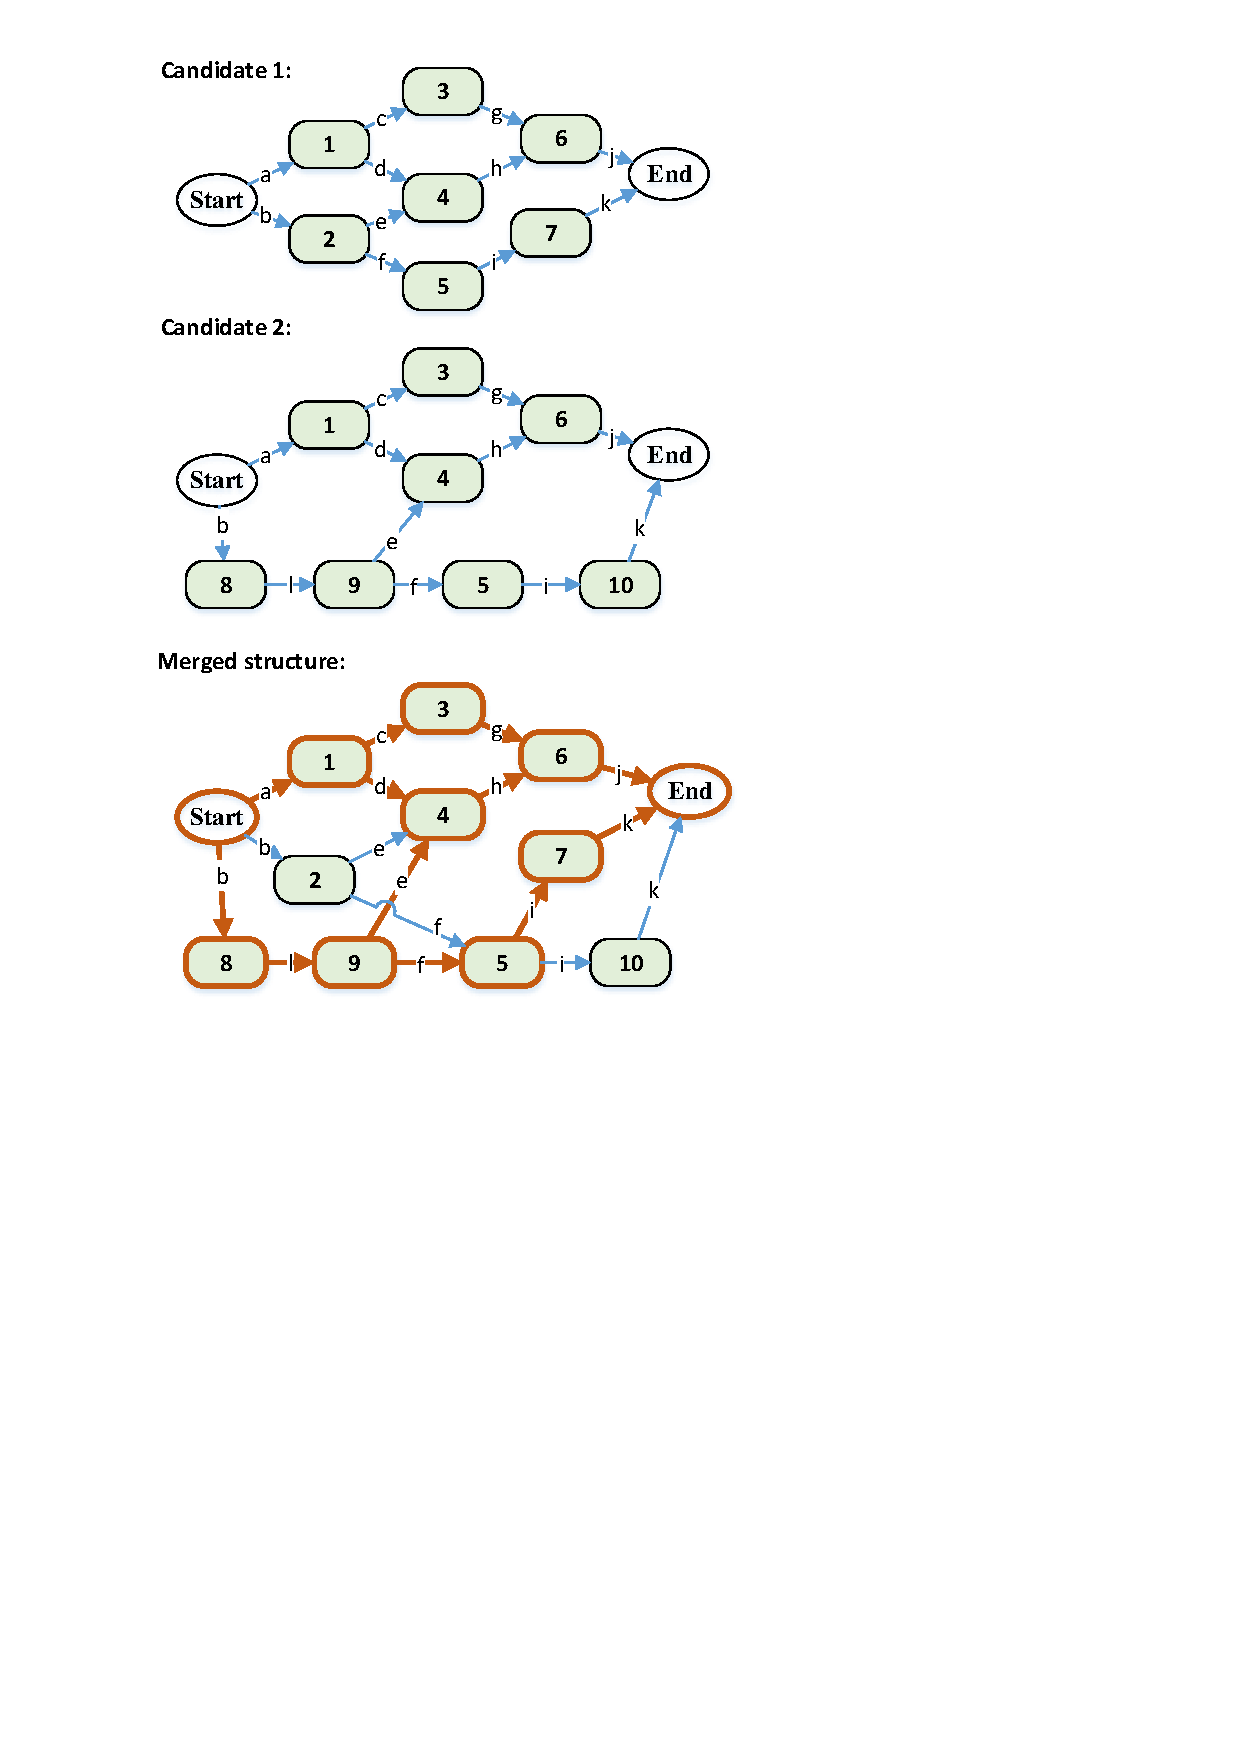
\includegraphics[width=8cm]{crossoverExample.pdf}}}
\caption{Example of the merge and extraction process used in the graph crossover operation.}
\label{fig:crossoverExample}
\end{figure}

\subsection{Fitness function}
The fitness function employed for the evolutionary process is based on the one presented in \cite{rodriguez2010composition}. It seeks to
produce solutions with the smallest possible number of service nodes and with the shortest possible paths from the start node to the
end node. The rationale behind this function is that it encourages features indicative of the quality of the overall composition \cite{rodriguez2010composition}:
the number of service nodes indicates the complexity of the overall composition (it should be as small as possible); the length of
the longest path from the start node to the end node indicates the execution time of the composition solution, with a shorter
path indicating more parallelisation of tasks and consequently a lower execution time. The fitness function is formally described as follows:

\begin{equation}
 fitness_i = \omega_1 \cdot \frac{1}{runPath_i} + \omega_2 \cdot \frac{1}{\#atomicProcess_i}
\end{equation}

\noindent where $ \omega_1 + \omega_2 = 1$, $runPath_i$ is the longest path from the start node to the end node of a solution $i$ (measured using a longest
path algorithm), and $\#atomicProcess_i$ is the total number of service nodes included into a solution $i$. In the original paper, the fitness function also
presents a third criterion measuring the degree of satisfaction of the inputs for each service node in the solution. In our case, however, this is not
necessary, since the graph building algorithm used throughout the evolution process ensures that the inputs of each service included in a solution are
always fully satisfied.

\begin{table*}[ht]
\footnotesize
\centerline{
\def\arraystretch{1.5}
\begin{tabular}{c|c|c|c|c|c|c|}
\cline{2-7}
\textbf{}                           & \multicolumn{3}{c|}{\textbf{GraphEvol}}                                                              & \multicolumn{3}{c|}{\textbf{GP Approach}}                                                            \\ \hline
\multicolumn{1}{|c|}{\textbf{Task}} & \textbf{Time (ms)} & \textbf{runPath} & \multicolumn{1}{c|}{\textbf{\#atomicProcess}} & \multicolumn{1}{c|}{\textbf{Time (ms)}} & \textbf{runPath} & \textbf{\#atomicProcess} \\ \hline
\multicolumn{1}{|c|}{OWL-S TC-1}    & $469.60 \pm 108.10$     & $1.00 \pm 0.00$       & $1.00 \pm 0.00$                                    & $749.00 \pm 364.10$                          & $1.00 \pm 0.00$       & $1.00 \pm 0.00$               \\ \hline
\multicolumn{1}{|c|}{OWL-S TC-2}    & $326.73 \pm 29.07$      & $1.00 \pm 0.00 \downarrow$       & $1.00 \pm 0.00\downarrow$                                    & $484.50 \pm 139.20$                          & $2.00 \pm 0.00$       & $2.00 \pm 0.00$               \\ \hline
\multicolumn{1}{|c|}{OWL-S TC-3}    & $517.17 \pm 99.98$      & $2.00 \pm 0.00$       & $2.00 \pm 0.00$                                    & $473.60 \pm 76.19$                           & $2.00 \pm 0.00$       & $2.00 \pm 0.00$               \\ \hline
\multicolumn{1}{|c|}{OWL-S TC-4}    & $674.23 \pm 107.50$     & $2.00 \pm 0.00\downarrow$       & $4.00 \pm 0.00\downarrow$                                    & $3010.20 \pm 422.91$                         & $2.20 \pm 0.40$       & $5.70 \pm 1.19$               \\ \hline
\multicolumn{1}{|c|}{OWL-S TC-5}    & $472.23 \pm 46.33$      & $1.00 \pm 0.00$       & $3.00 \pm 0.00\downarrow$                                    & $1098.30 \pm 240.72$                         & $1.00 \pm 0.00$       & $3.30 \pm 0.46$               \\ \hline
\multicolumn{1}{|c|}{WSC 2008-1}    & $699.43 \pm 93.79$      & $3.00 \pm 0.00\downarrow$       & $10.00 \pm 0.00\downarrow$                                   & $6919.70 \pm 1612.99$                        & $6.00 \pm 1.26$       & $15.8 \pm 5.71$               \\ \hline
\multicolumn{1}{|c|}{WSC 2008-2}    & $734.63 \pm 102.84$     & $3.00 \pm 0.00\downarrow$       & $5.00 \pm 0.00\downarrow$                                    & $11137.20 \pm 3106.75$                       & $3.50 \pm 0.67$       & $6.00 \pm 0.89$               \\ \hline
\multicolumn{1}{|c|}{WSC 2008-5}    & $918.40 \pm 120.13$     & $8.00 \pm 0.00\downarrow$       & $20.00 \pm 0.00\downarrow$                                   & $95390.20 \pm 43521.30$                      & $9.20 \pm 2.96$       & $49.90 \pm 16.84$             \\ \hline
\end{tabular}}
\caption{Mean execution times, longest path lengths, and number of service nodes for each task in GraphEvol and GP \protect\cite{rodriguez2010composition}.}
\label{resultsTable}
\end{table*}

\section{Experiment Design}\label{experimentdesign}
Experiments were carried out to compare the performance of GraphEvol against the GP approach presented in \cite{rodriguez2010composition}, seeking to validate
the hypothesis that the execution time, total number of service nodes, and longest path in the resulting compositions will be similar or smaller to those produced
by GP. The validation of this hypothesis would indicate that GraphEvol is a suitable alternative to Web service composition using GP, matching the effectiveness of the
latter while at the same time providing the benefits of a direct solution representation. The authors who introduced the GP approach also presented experimental
results of that method's application to two datasets using a variety of composition tasks, thus those results will be used as the basis of this comparison.

\subsection{Datasets}
The datasets employed in this experiments were OWL-S TC V2.2 \cite{kuster2008opossum} and WSC 2008 \cite{bansal2008wsc}, both of which present service collections
of varying sizes accompanied by ontologies. These ontologies detail how the input and output types of the services in the collection relate to each other at
a conceptual level. For example, suppose the ontology contains information stating that an \textit{integer} is a type of \textit{number}. Given this information,
if a service is annotated as requiring a \textit{number} as an input and another is annotated as producing an \textit{integer} as an output, then one may infer
that the \textit{integer} output can be used to fulfil the \textit{number} input. As shown by this example, the advantage of having such information encoded in an
ontology is that it enables the matching of data types that are named differently but are nevertheless compatible. Tasks 1--5, which are outlined in \cite{rodriguez2010composition},
were used when to test GraphEvol against the OWL-S TC dataset; tasks WSC 2008-1, WSC 2008-2, and WSC 2008-5 were used for testing against the WSC 2008 dataset.

\subsection{Parameters}
Testing was conducted using a personal computer with an Intel Core i7-4770 CPU (3.4 GHz), and 8 GB RAM. To match the GP approach, a population of 200 candidates was
evolved during 20 generations for each composition task, and this process was repeated over 30 independent runs. The fitness function weights $\omega_1$ and $\omega_2$
were both set to 0.5, the mutation probability to 0.05, and the crossover probability to 0.5. Individuals were chosen for breeding using tournament selection with a 
tournament size of 2, mirroring the design of the experiment conducted by the authors of the GP approach \cite{rodriguez2010composition}.

\section{Results}\label{results}

%\subsection{Overall Results}
Experiment results for GraphEvol are presented in columns 1, 2, and 3 of Table \ref{resultsTable}, side by side with the previously published GP results. Column 1 displays the mean execution time for GraphEvol in milliseconds; column 2 presents the mean length of the longest path in a run's best solution; column 3 shows the mean number of service nodes included in a run's
best solution. Means are accompanied by their respective standard deviations, and all values in the table are rounded to 2 decimal points of precision. While the two approaches were executed in different platforms, meaning that it is not possible to
perform a direct comparison on execution time, the large time gap when executing tasks OWL-S TC-4, WSC 2008-1, WSC 2008-2, and WSC-2008-3 provides strong evidence that the GraphEvol approach can handle certain service collections more effectively than the GP approach. For the other tasks, on the other hand, there is no obvious time difference.

Since both approaches were tested using the same datasets and tasks, as well as employing equivalent fitness functions during the evolutionary process, it is possible to perform a direct comparison on the longest path lengths and overall number of nodes of the solutions produced. Unpaired t-tests at 0.05 significance level were conducted to verify whether there are statistically
significant differences between the results produced by each technique. Such differences are denoted using $\uparrow$ for significantly higher results and $\downarrow$ for significantly lower. The tests revealed that GraphEvol yielded solutions with equivalent or significantly smaller longest paths and numbers of nodes, that is, the quality of the solutions produced by GraphEvol always matched or surpassed that of the solutions produced by GP. These results establish the GraphEvol approach as a powerful alternative when performing fully automated Web service composition.

%\subsection{Discussions}

\section{Conclusions}\label{conclusions}
This work presented GraphEvol, an evolutionary computation technique aimed at performing fully automated Web service composition using graph representations for solutions, as opposed to encoding them into tree or vector representations. A graph building algorithm was proposed for generating the initial population, and variations of it were employed during the evolutionary process. The traditional mutation and crossover operations were modified to work with graph candidates, involving graph merging and traversal procedures. Finally, experiments were conducted comparing GraphEvol to an analogous GP approach. Results showed that the quality of the results produced by GraphEvol always matched or surpassed those produced by GP, requiring roughly the same or less execution time. It is believed that improvements can be made to the crossover operator (e.g. restrict crossover operation to graphs that present a certain degree of similarity), therefore research on this topic is a natural future development.
Another possibility is the execution of additional tests, this time expanding the experiment design to include fitness functions that measure formal Quality of Service (QoS) attributes \cite{jaeger2007qos} of candidate compositions.

%% The file named.bst is a bibliography style file for BibTeX 0.99c
\clearpage
\bibliographystyle{named}
\bibliography{ijcai15}

\end{document}

